\documentclass{beamer}

\input{../preambulo/inputenc.tex}
\input{../preambulo/fuente.tex}
\input{../preambulo/spanish.tex}
\input{../preambulo/tikz.tex}
\input{../preambulo/matematica.tex}
\input{../preambulo/colors.tex}
\input{../preambulo/flotantes.tex}
\input{../preambulo/beamer_zub.tex}
\input{../preambulo/paquetes.tex}
\usepackage{ccicons}
% \ccPublicDomain

\newcommand{\etal}{{\it et al.}}
\newcommand{\ie}{{\it i. e.}}
\newcommand{\zlink}[1]{\href{#1}{\color{celeste}\faExternalLink*}}


\graphicspath{{../img/}{img/}}
\framebg{bg/pizarron3.png} 

\begin{document}

\newcommand\CC{}

\begin{zframe}{}
\path(cp) ++(3,0) node(I)[]{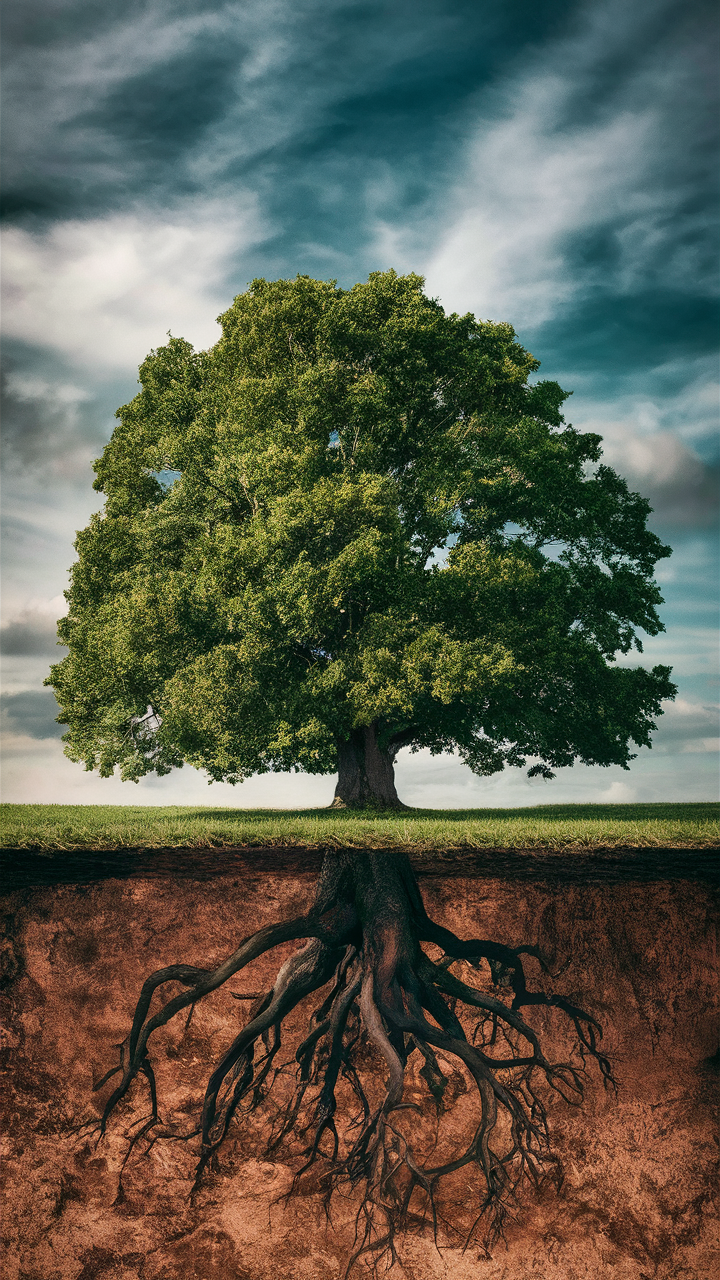
\includegraphics[width=5cm]{ideogram/raices.png}};
\path(c2|-I.north) ++(0,-1) node(A)[anchor=north,align=left]{
  \color{verde} \large\textbf{Métodos Computacionales}\\[3mm]  
  \color{celeste} \textbf{Búsqueda de raíces}\\[2mm]  
  \color{lila} \textit{Agosto 6, 2025}
};
\normalsize
\path(A.west|-I.south) ++(0,1) node(B)[anchor=south west,align=left]{
  S. Alexis Paz\\[5mm]

\includegraphics[width=3cm]{logos/DQTC_orange.png}};
 
\path(I.south east) ++(0,.2) node[anchor=north east]{
  \tiny hecho con \href{https://ideogram.ai/g/D3j2DRuIR7W-Qz3f-qOLVg/1}{ideogram}};
                        
\end{zframe}

\renewcommand\CC{
  \path(se) node[anchor=south east]{\tiny\color{gray} MC2025 - S.A.Paz};
}
\begin{zframe}{}
  
\path(t-|np) ++(0,.5) node(T)[anchor=north,text width=11cm]{
  \centerline{\Large \color{verde} ¿$L$ tal que $f(L)=0$?}\\[4mm]
 Si podemos determinar las raíces de una ecuación también podemos determinar
   máximos y mínimos, valores propios de matrices, resolver sistemas de
   ecuaciones lineales y diferenciales, etc...};

\path(T.south) ++(0,-.5) node(T)[theo,anchor=north,text width=12cm]{
\\[1mm]
Sea ${f:\mathbb{R}\rightarrow\mathbb{R}}$ continua en ${[a,b]}$ y ${m\in\mathbb{R}}$
tal que ${f(a)<m<f(b)}$, entonces existe ${x\in(a,b)}$ tal que ${f(x)=m}$.};
\path(T.north west) node(H)[theohead,anchor=north west]{Teorema del valor intermedio};

           
\path(T.south east) ++(0,-.5) node(T)[theo,anchor=north east,align=left]{
\\[1mm]
Si $f(a)$ y $f(b)$ tienen signos opuestos,\\ entonces $f$ tiene una raíz ${L\in(a,b)}$.
};
\path(T.north east) node(H)[theohead,anchor=north east,fill=black]{\color{naranja}\it corolario};
 
\path(c3) ++(-.6,-.5) coordinate(scope);
\begin{scope}[x=1cm,y=0.8cm,shift=(scope),thick]
\zcuad{0,0}{-2,-1}{3,2} %\showcuad
\draw[style=help lines, ystep=1, xstep=1] (sw) grid (ne);
\draw[->] (w) -- (e);% node[right] {$x$};

\draw[amarillo, domain=-2:3] plot[smooth,yrange=-1:2,id=f] function{sin(.5*x)+.5*x};
\draw[dashed,celeste,->] (-.8,0)	node[above]{$a$} -- (-.8,-1) node[right]{$f(a)$};
\draw[dashed,celeste,->] (2,0) node[above right]{$b$} -- (2,1.9) node[below right]{$f(b)$};
\draw[dashed,rosa,->] (1,0) node[above right]{$x$} -- (1,1) node[above left]{$m$};
\end{scope}

\end{zframe}        

\begin{zframe}{}
 
\path(nw) ++(.2,-.6) node(T)[alg,text width=12cm]{\vspace{-2mm}
\begin{enumerate}[\color{rosa}1.]
\item Elige $\ab[a,b]$ tal que $f(a)f(b)<0$ y una tolerancia $\epsilon_T$.\\
\item Calcula $x\Leftarrow(a+b)/2$.
\item Si $|b-a|<\epsilon_T$, terminar. {\color<2->{rosa} La raíz es $x$}.
\item Si $f(a)f(x)\leq0$ entonces $b\Leftarrow x$, sino $a\Leftarrow x$.
\item Volver al paso 2.
\end{enumerate}};
\path(T.north west) node(H)[alghead]{Bisección};

\draw<2->[->,ultra thick,verde](T.south west) ++(0.4,0.3) -- ++(-0.2,0) -- ++(0,2.5) -- ++(0.23,0);
% \draw<2>[-,ultra thick,amarillo](T.center) ++(-1.1,-0.1) -- ++(0,0.2) -- ++(2.1,0) node[pos=0.5,above=-.1]{\scriptsize falso} -- ++(0,-0.2) ;
\draw<2->[-,ultra thick,amarillo](T.center) ++(-2.7,-0.1) -- ++(0,0.2) -- ++(1.5,0) node[pos=0.5,above=-.1]{\scriptsize verdadero}     -- ++(0,-0.2) ;

\draw<2->[-,ultra thick,amarillo](T.center) ++(-5.1,-0.15) circle(.3);
\draw<2->[-,ultra thick,amarillo](T.center) ++(-5.1,-0.9) circle(.3);

\draw<2->[-,ultra thick,amarillo](T.center) ++(0.945,-0.9) -- ++(0,0.2) -- ++(1.2,0) node[pos=0.5,above=-.1]{\scriptsize falso} -- ++(0,-0.2) ;
\draw<2->[-,ultra thick,amarillo](T.center) ++(-1.05,-0.9) -- ++(0,0.2) -- ++(1.2,0) node[pos=0.5,above=-.1]{\scriptsize verdadero}  -- ++(0,-0.2) ;
                        
\path<3>(hr)  ++(0.7,1.3)  node(D0)[verde]{\textbf{Inicio}};
\path<3>(D0)  ++(0,-1)  node(D1)[fill=verde,draw=verde,rectangle,thick,text opacity=1,fill opacity=0.4]{$x\Leftarrow(a+b)/2$};
\path<3>(D1)  ++(0,-1.2)  node(D2)[fill=amarillo,draw=amarillo,inner sep=0,diamond,aspect=3,thick,text opacity=1,fill opacity=0.4]{$|b-a|<\epsilon_T$?};
\path<3>(D2)  ++(0,-1.4)  node(D3)[fill=amarillo,draw=amarillo,inner sep=0,diamond,aspect=3,thick,text opacity=1,fill opacity=0.4]{$f(a)f(x)\leq0$?};
\path<3>(D3) ++(-1,-1.2) node(D4a)[fill=verde,draw=verde,minimum height=2ex,rectangle,thick,text opacity=1,fill opacity=0.4]{$b\Leftarrow x$};
\path<3>(D3)  ++(1,-1.2) node(D4b)[fill=verde,draw=verde,minimum height=2ex,rectangle,thick,text opacity=1,fill opacity=0.4]{$a\Leftarrow x$};
\path<3>[<-,ultra thick,verde](D2) ++(-1.4,-.8) node(D5)[verde]{\textbf{Fin}};

\draw<3>[->,ultra thick,verde](D0) -- (D1);
\draw<3>[->,ultra thick,verde](D1) -- (D2);
\draw<3>[->,ultra thick,verde](D2) -- (D3) node[pos=0.5,right]{\small no};  
\draw<3>[->,ultra thick,verde,shorten >=-8](D2) -- (D5) node[pos=0.5,below right=-.2]{\small si}; 
\draw<3>[->,ultra thick,verde](D3) -- (D4a) node[pos=0.5,above left=-.2]{\small si};
\draw<3>[->,ultra thick,verde](D3) -- (D4b) node[pos=0.5,above right=-.2]{\small no};

\draw<3>[->,ultra thick,verde](D4a.south) -- ++(0,-0.2) -| (D4b) --  (D4b|-D4a.south) ++(0,-0.2) -- ++(1,0) |- (D1);
                        
\path(hl) ++(1.0,-2.8) coordinate(scope);
\begin{scope}[x=1cm,y=0.8cm,shift=(scope),thick]
\zcuad{-2,0}{-3,-2}{3,3} %\showcuad
\draw[style=help lines, ystep=1, xstep=1] (sw) grid (ne);
\draw[->] (w) -- (e) node[right] {$x$};

\draw[color=amarillo, domain=-3:3] plot[smooth,id=parabola,yrange=-2:3] function{sin(2*x)+x} node
[above,yshift=-3,xshift=-25] {$f(x)=\sin(x)+x$};


% xticks and yticks
% {\scriptsize
% \foreach \x in {-3,-2,...,3}  \path(o-|{(\x,0)}) node[below]{\x};
% \foreach \y in {-4,-3,...,4} \path(o|-{(0,\y)}) node[left]{\y};
% }

% generate and plot another a curve y = 0.1 x^2 + 2.5
% this generates the files figure.parabola.gnuplot and figure.parabola.table 
\ifundef{\globalxa}{\gdef\globalxa{-1.5}}{}
\ifundef{\globalxb}{\gdef\globalxb{1.2}}{}
\pgfmathtruncatemacro\N{7}
\foreach \m in {4,5,...,\N}{ 
\only<\m>{
                                              
  % Punto b
  \pgfmathsetmacro\x{\globalxb}
  \pgfmathsetmacro\y{sin(2*\x*180/3.1415)+\x}
  \pgfmathsetmacro\la{sign(\y)*(-7)}

  \fill[verde] (\x,\y) circle(0.1cm);
  \draw[verde,dashed] (\x,0) -- (\x,\y) node[pos=0,yshift=\la]{$b$};
  \draw[verde,dashed] (o|-{0,\y}) -- (\x,\y) node[pos=0,left]{$f(b)$};
    
  % Punto a
  \pgfmathsetmacro\xx{\globalxa}
  \pgfmathsetmacro\yy{sin(2*\xx*180/3.1415)+\xx}
  \pgfmathsetmacro\lb{sign(\yy)*(-7)}
  
  \fill[verde] (\xx,\yy) circle(0.1cm);
  \draw[verde,dashed] (\xx,0) -- (\xx,\yy) node[pos=0,yshift=\lb]{$a$};
  \draw[verde,dashed] (o|-{0,\yy}) -- (\xx,\yy) node[pos=0,left]{$f(a)$};
 
  % Etiquetas
  \path(3.8,2.9) node(ab)[anchor=north west,align=left]{
   {\color{rosa} 1.} a=\xx\\
    \hspace{2ex}     b=\x};
  \pgfmathsetmacro\iter{int(\m-1))}
  \path(6.5,3.0) node(Bi)[rectangle,draw=white,anchor=north west]{
    Iteración \iter};
  \path(Bi.south) node[anchor=north]{
    $\epsilon_T=0.4$};

  % Distancia
  \pgfmathsetmacro\d{\x-\xx}
  \path(3.8,-0.7) node[anchor=south west,align=left]{
    {\color{rosa} 3.} Convergencia:\\
    \hspace{2ex}$b-a=\d$
  };


  % Punto c
  \pgfmathsetmacro\xc{(\xx+\x)*.5}
  \pgfmathsetmacro\yc{sin(2*\xc*180/3.1415)+\xc}
  \pgfmathsetmacro\lc{sign(\yc)*(-7)}
  
  \fill[celeste] (\xc,\yc) circle(0.1cm);
  \draw[celeste,dashed] (\xc,\yc) -- (\xc,0) node[pos=1,yshift=\lc]{$x$};
  \draw[celeste,dashed] (o|-{0,\yc}) -- (\xc,\yc) node[pos=0,left,yshift=-5]{$f(x)$};

  \path(3.8,1.1) node(x)[anchor=west,align=left]{
  {\color{rosa} 2.} $x=\xc$};

  \pgfmathsetmacro\test{sign(\yc*\yy)}
  \ifthenelse{\test>0}{
    \global\let\globalxa=\xc
    \path(3.8,-1.4) node[anchor=west,align=left]{
     {\color{rosa} 4.} $f(a)f(x)>0$};
    \draw[rosa] (ab.0) ++(0,.4) edge[<-,>=stealth,double=black,double distance=1pt,bend left] (x.15);
  }{
    \global\let\globalxb=\xc
    \path(3.8,-1.4) node[anchor=west,align=left]{
      {\color{rosa} 4.} $f(a)f(x)<0$};
    \draw[rosa] (ab.0) ++(0,-.4)  edge[<-,>=stealth,double=black,double distance=1pt,bend left] (x.15);
  }


}
}

\only<\N>{
  \global\let\globalxa\undefined
  \global\let\globalxb\undefined
}
   

     
\path(-1,2.8) node(B)[anchor=north west,align=left]{
  $L$=0};
\draw[<-,dashed](B) to[bend right] (0,0);
                               
\end{scope}
 
\end{zframe}
                                                                 
\begin{zframe}{}
\path(nw) ++(.2,-.6) node(T)[alg,text width=12cm]{\vspace{-2mm}
\begin{enumerate}[\color{rosa}1.]
\item Elige $\ab[a,b]$ tal que $f(a)f(b)<0$ y una tolerancia $\epsilon_T$.\\
\item Calcula $x\Leftarrow(a+b)/2$.
\item Si $|b-a|<\epsilon_T$, terminar. La raíz es $x$.
\item Si $f(a)f(x)\leq0$ entonces $b\Leftarrow x$, sino $a\Leftarrow x$.
\item Volver al paso 2.
\end{enumerate}}; 
\path(T.north west) node(H)[alghead]{Bisección};
 
\path(vl) ++(3,1) node(A)[draw=lila,fill=black,text width=5cm]{
  \vspace{-2.5ex}\inputminted[bgcolor=black]{python}{code/bisec.py}\vspace{-4ex}};
\path(A.west) ++(0,0) node[anchor=west,opacity=0.1]{
\includegraphics[width=5cm]{python_logo.png}};

\end{zframe}
          
\begin{zframe}[<1>]{}
 
\path(nw) ++(.2,-.6) node(T)[alg,text width=12cm]{\vspace{-2mm}
\begin{enumerate}[\color{rosa}1.]
\item Elige $\ab[a,b]$ tal que $f(a)f(b)<0$ y una tolerancia $\epsilon_T$.\\
\item Calcula $x\Leftarrow(a+b)/2$.
\item Si $|b-a|<\epsilon_T$, terminar. La raíz es $x$.
\item Si $f(a)f(x)\leq0$ entonces $b\Leftarrow x$, sino $a\Leftarrow x$.
\item Volver al paso 2.
\end{enumerate}};  
\path(T.north west) node(H)[alghead]{Bisección};
 

\path(T.south west) ++(2,-.5) node(A)[align=left,anchor=north west]{
\Large ¿Error?\\
  \only<2>{\hspace{1cm} {\small ABSOLUTO:} \hspace{1cm} $\ds\epsilon_n=\left|x_n-L\right|$}\\[1mm]
  \only<2>{\hspace{1cm} {\small RELATIVO:} \hspace{1cm} $\ds\tilde\epsilon_n=\left|x_n-L\right|/x_n$ }\\
};

\path(A.south west) ++(0,.1) node[align=left,anchor=north west]{
\Large ¿Convergencia?\\[1mm]
};

\end{zframe}
  
\begin{zframe}{}
 
\path(nw) ++(.2,-.6) node(T)[alg,text width=12cm]{\vspace{-2mm}
\begin{enumerate}[\color{rosa}1.]
\item Elige $\ab[a,b]$ tal que $f(a)f(b)<0$ y una tolerancia $\epsilon_T$. {\hspace{1cm}\hfill\color{verde}${n\Leftarrow 0}$}\\
\item Calcula $x_{\color{verde}n}\Leftarrow(a+b)/2$. \\
\item Si $|b-a|<\epsilon_T$, terminar. La raíz es $x_{\color{verde}n}$.
\item Si $f(a)f(x_{\color{verde}n})\leq0$ entonces $b\Leftarrow x_{\color{verde}n}$, sino $a\Leftarrow x_{\color{verde}n}$.
\item Volver al paso 2. \hfill{\hspace{1cm}\color{verde}${n\Leftarrow n+1}$}
\end{enumerate}};
\path(T.north west) node(H)[alghead]{Bisección};
 

\path(T.south west) ++(2,-.5) node(A)[align=left,anchor=north west]{
\Large ¿Error?\\
  \only<2>{\hspace{1cm} {\small\color{naranja} ABSOLUTO:} \hspace{1cm} $\ds\epsilon_n=\left|x_n-L\right|$}\\[1mm]
  \only<2>{\hspace{1cm} {\small\color{naranja} RELATIVO:} \hspace{1cm} $\ds\tilde\epsilon_n=\left|x_n-L\right|/x_n$ }\\
};

\path(A.south west) ++(0,.1) node(A)[align=left,anchor=north west]{
\Large ¿Convergencia?\\[1mm]
  \only<2>{\hspace{1cm} $\ds\lim_{n\to\infty}x_n=L$}\\[2mm]
  \only<2>{\hspace{1cm} $\ds\epsilon_{n+1}=C\epsilon_n^p\quad;\quad n\to\infty$}
};

\draw<2>[->,ultra thick](A.west) ++(.8,-.75) -- ++(-1.3,0) node[above left,rotate=30]{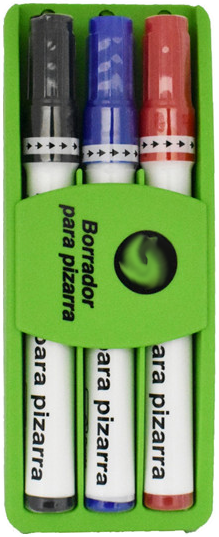
\includegraphics[width=6mm]{marcadores.png}};
 
\path(A.east) ++(.4,-.2) node[align=left,anchor=west]{
  \only<2>{$p\to${\small\color{naranja} ORDEN}}\\[2mm]
  \only<2>{$C\to${\small\color{naranja} VELOCIDAD}}
};
 
          

\end{zframe}
     

\begin{zframe}{}
           
\path(t-|np) ++(0,0.5) node(T)[theo,anchor=north,text width=12cm, inner sep=6,align=center]{\\[1mm]
Sea ${f:\mathbb{R}\rightarrow\mathbb{R}}$ una función
diferenciable $k$ veces en el punto ${a\in\mathbb{R}}$. Entonces
existe ${g_k:\mathbb{R}\rightarrow\mathbb{R}}$ tal que
\begin{equation*}
\ds f(x){\color{celeste}=}f(a)+f'(a)(x-a)+\cdots+\frac{f^{(k)}(a)}{k!}(x-a)^{k}+{\color{celeste}g_k(x)(x-a)^k}
\end{equation*}
con $\lim_{x\to a}g_k(x)=0$.};
\path(T.north west) node(H)[theohead,anchor=west]{Teorema de Taylor};
\path(T.north east) node(H)[theohead,anchor=east,fill=black]{\color{white}\it forma de Peano};
               
\path(T.south) ++(0,-.4) node(T)[theo,anchor=north,text width=12cm, inner sep=6,align=center]{\\[1mm]
Sea ${f:\mathbb{R}\rightarrow\mathbb{R}}$ una función
diferenciable $k+1$ veces en el intervalo abierto entre $a$ y $x$ con $f^{(k+1)}$ continua en el cerrado. Entonces
\begin{equation*}
\ds f(x){\color{celeste}=}f(a)+f'(a)(x-a)+\cdots+\frac{f^{(k)}(a)}{k!}(x-a)^{k}+{\color{celeste}\frac{f^{(k+1)}(\xi)}{(k+1)!}(x-a)^{k+1}}
\end{equation*}
con $\xi$ entre $x$ y $a$.};
\path(T.north east) node(H)[theohead,anchor=east,fill=black]{\color{white}\it forma de Lagrange};
            
\path(wp) ++(.2,0) node(I)[anchor=west,inner sep=0]{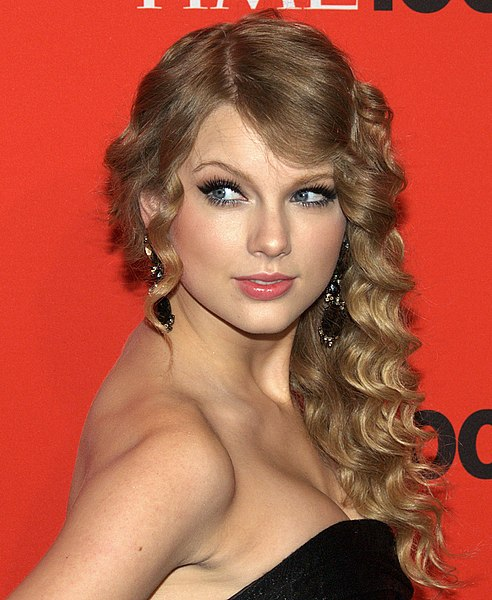
\includegraphics[width=1.4cm]{taylor.jpg}};
\path(I.south east) ++(0,0) node[scale=0.5,anchor=south east,align=right,inner sep=0]{
  \tiny \href{https://commons.wikimedia.org/wiki/File:5.3.10TaylorSwiftByDavidShankbone.jpg}{D. Shankbone, CC BY 3.0}
  };
\path(I.east) ++(0,0) node(I)[anchor=west,inner sep=0]{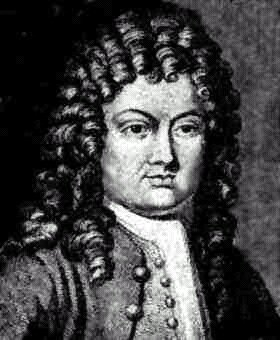
\includegraphics[width=1.4cm]{BTaylor.jpg}};
\path(I.south east) ++(0,0) node[scale=0.5,inner sep=0,anchor=south east]{\tiny\ccPublicDomain};
                                       
\end{zframe} 


\begin{zframe}{} 
      
\path<1>(t-|np) ++(0,0) node(T){Aproxima mejor en las cercanías de $a$};
\path<1>(T.south) ++(0,-0.2) node(T)[anchor=north]{
  $\ds f(x)=f(a)+f'(a)(x-a)+\cdots+\frac{f^{(k)}(a)}{k!}(x-a)^{k}+{\color{celeste}\frac{f^{(k+1)}(\xi)}{(k+1)!}(x-a)^{k+1}}$};

\path<2>(t-|np) ++(0,0) node(T){Usualmente escribimos:};
\path<2>(T.south) ++(0,-0.2) node(T)[anchor=north]{
  $\ds f(x)=f(a)+f'(a)(x-a)+\cdots+\frac{f^{(k)}(a)}{k!}(x-a)^{k}+{\color{celeste}O\ab((x-a)^{k+1})}$};

\path<2>(T.south east) ++(-1.6,0.1) node(T)[anchor=north,rotate=10,verde,draw,ellipse,align=center]{próxima\\ clase};
                          
\path<3>(t-|np) ++(0,0) node(T){Y para peor casi siempre hacemos\ldots};
\path<3>(T.south) ++(0,-0.2) node(T)[anchor=north]{
  $\ds f(x+h)=f(x)+f'(x)h+\cdots+\frac{f^{(k)}(x)}{k!}h^{k}+{\color{celeste}O\ab(h^{k+1})}$};

\path<3>(T.south east) ++(-.3,0.1) node(T)[anchor=north,rotate=10,amarillo,draw,align=center]{$x\gets x+h$\\$a\gets x$};
                          
\path<-2>(hl) ++(-0.5,0.5) node(T)[align=left]{
  {\color{celeste}$a$} es donde ``estoy''\\{\color{verde}$x$} es donde ``aproximo''};
\path<3>(hl) ++(-0.5,0.5) node(T)[align=left]{
  {\hspace{6mm} \color{celeste}$x$} es donde ``estoy''\\{\color{verde}$x+h$} es donde ``aproximo''};
                          
\path(vl) ++(-1.5,1.3) coordinate(scope);
\begin{scope}[scale=1.3,shift=(scope),thick]
\zcuad{0,-.5}{-1,-2}{3,2} %\showcuad
\draw[style=help lines, ystep=1, xstep=1] (sw) grid (ne);
\draw[->] (w) -- (e) node[right] {$x$};

\draw[color=amarillo, domain=-1:3] plot[smooth,id=parabola] function{(erf(x)+sin(x)+x)*.5};

\path(o) ++(1,0) coordinate(a);
\fill[celeste](a) ++(0,1.85) circle(3pt);

\draw<-2>[<-,ultra thick,celeste,dashed] (a) -- ++(0,-.7) node(B)[below]{\Large $a$};
\draw<3>[<-,ultra thick,celeste,dashed] (a) -- ++(0,-.7) node(B)[below]{\Large $x$};

\draw<-2>[->,ultra thick,verde,dashed] (a) ++(0.2,.5) node(B)[above]{\Large $x$} -- ++(0,-.5) ;
\draw<3>[->,ultra thick,verde,dashed]  (a) ++(0.2,.5) node(B)[above]{\Large $x+h$} -- ++(0,-.5) ;

% FIXME: Esto es aproximado
\draw[dashed,color=celeste, domain=-1:3, yrange=-2:2] plot[smooth,id=parabola] function{0.9*(x-1)+1.35};
\draw[dashed,color=celeste, domain=-1:3, yrange=-2:2] plot[smooth,id=parabola] function{-2*(x-1)**2+1.35};
% \draw[color=celeste, domain=-3:3] plot[smooth,id=parabola] function{4*(x-1)**3+2*(x-1)**2+1.3};
\draw[very thick, color=celeste, domain=-3:3, yrange=-2.5:2] plot[smooth,id=parabola] function{0.9*(x-1)-2*(x-1)**2+1.35};

\end{scope}
\end{zframe} 
      
                                                  
\begin{zframe}{}
   
\path(nw) ++(.2,-.6) node(T)[alg,text width=12cm]{\\[1mm]
\begin{enumerate}[\color{rosa}1.]
\item Elige $x_n$ y una tolerancia $\epsilon_T$ para el resultado. ${n=0}$.\\
\item Calcula ${x_{n+1}=x_n-f(x_n)/f'(x_n)}$.
\item Si ${|x_{n+1}-x_n|<\epsilon_T}$, terminar. La raíz es: $x_{n+1}$.
\item Volver al paso 2, ${n\Leftarrow n+1}$.
\end{enumerate}};
\path(T.north west) node(H)[alghead]{Newton-Rapshon};
           
\path(T.south west) ++(0,-0.5) node(T)[alg,align=left,text width=12cm]{\\[1mm]
\begin{enumerate}
\item[\color{rosa}3.] Si $|(x_{n+1}-x_n)/x_n|<\epsilon_T$, terminar. La raíz es: $x_{n+1}$.
\end{enumerate}};
\path(T.north east) node(H)[alghead,anchor=north east,fill=black]{\color{white}\it variante};
                     
\path(T.south west) ++(0,-0.5) node(T)[alg,align=left,text width=12cm]{\\[1mm]
\begin{enumerate}
\item[\color{rosa}3.] Si $|f(x_{n+1})|<\epsilon_T$, terminar. La raíz es: $x_{n+1}$.
\end{enumerate}};
\path(T.north east) node(H)[alghead,anchor=north east,fill=black]{\color{white}\it variante};
                             
\end{zframe}     


\begin{zframe}{}
\ifundef{\globalxa}{\gdef\globalxa{-0.72}}{}
 
\path(np) ++(0,-0.5) node[verde,anchor=north]{\Large Newton-Raphson};
\path(hl) ++(1.0,0) coordinate(scope);

\begin{scope}[x=1cm,y=0.8cm,shift=(scope),thick]

% Definir
\path(-2,0) coordinate(O);
\path(3,4) coordinate(K1);          % Esquina del cuadrante 1
\path(K1-|{(-3,0)}) coordinate(K2); % Esquina del cuadrante 2
\path(K2|-{(0,-4)}) coordinate(K3); % Esquina del cuadrante 3

% Emergentes
\path(K3-|K1) coordinate(K4);       % Esquina del cuadrante 4
\path(O-|K1) coordinate(xp);       % Punta de eje +x
\path(O-|K2) coordinate(xn);       % Punta de eje -x
\path(O|-K1) coordinate(yp);       % Punta de eje +y
\path(O|-K3) coordinate(yn);       % Punta de eje -y


% grid
\draw[style=help lines, ystep=1, xstep=1] (K3) grid (K1);

% axes
\draw[->] (xn) -- (xp) node[right] {$x$};
% \draw[->] (yn) -- (yp) node[right] {$y$};

% xticks and yticks
% {\scriptsize
% \foreach \x in {-3,-2,...,3}  \path(O-|{(\x,0)}) node[below]{\x};
% \foreach \y in {-4,-3,...,4} \path(O|-{(0,\y)}) node[left]{\y};
% }

% generate and plot another a curve y = 0.1 x^2 + 2.5
% this generates the files figure.parabola.gnuplot and figure.parabola.table 
\draw[color=amarillo, domain=-3:3] plot[smooth,id=parabola] function{sin(2*x)+x} node
[above,yshift=6,xshift=-15] {$f(x)=\sin(x)+x$};


\ifundef{\globalxa}{\gdef\globalxa{-0.8}}{}
\ifundef{\globalN}
  {\pgfmathtruncatemacro\N{4}}
  {\pgfmathtruncatemacro\N{\globalN}}
\foreach \n in {1,2,...,\N}{
\pgfmathsetmacro\m{int((\n-1))}
\only<\n>{

  % Punto x0
  \pgfmathsetmacro\x{\globalxa}
  \pgfmathsetmacro\y{sin(2*\x*180/3.1415)+\x}
  \pgfmathsetmacro\lc{sign(\y)*(-7)}

  \fill[verde] (\x,\y) circle(0.1cm);
  \draw[verde,dashed] (\x,0) -- (\x,\y) node[pos=0,yshift=\lc]{$x_\m$};
  \draw[verde,dashed] (O|-{0,\y}) -- (\x,\y) node[pos=0,left]{$f(x_\m)$};
       
  % Etiquetas
  \path(4,2) node[anchor=north west,align=left]{
    {\color{rosa} 1.} $x_\m=\x$};

  \path(6,4.5) node(Bi)[rectangle,draw=white,anchor=north west]{
    Iteración \n};
  \path(Bi.south) node[anchor=north]{
    $\epsilon_T=0.4$};



  % Tangente
  \pgfmathsetmacro\x{\globalxa}
  \pgfmathsetmacro\y{sin(2*\x*180/3.1415)+\x}
  \pgfmathsetmacro\a{2*cos(2*\x*180/3.1415)+1}
  \draw[color=celeste, domain=-3:3, yrange=-4:4] plot[smooth,id=parabola] function{(x-\x)*\a+\y};

  \pgfmathsetmacro\xx{-\y/\a+\x}
  \fill[celeste] (\xx,0) circle(0.1cm) node[above]{$x_\n$};
  \global\let\globalxa=\xx

  % Etiquetas
  \path(4,0.5) node[anchor=west,align=left]{
    {\color{rosa} 2.} $x_\n=\xx$};
 
  % Distancia
  \pgfmathsetmacro\d{abs(\x-\xx)}
  \path(4,-1.8) node[anchor=south west,align=left]{
    {\color{rosa} 3.} Convergencia:\\
    $\left|x_\m-x_\n\right|=\d$
  };        

}

}

\only<\N>{
  \global\let\globalxa\undefined
}
 
    
\end{scope}
 



\end{zframe}

\begin{zframe}{}

\path(nw) ++(1.2,-.2) node(A)[anchor=north west,text width=12cm]{\\[1mm]
\begin{itemize}
\item[\color{lila}$\bullet$] Necesitamos conocer la primera derivada de la funcion.
\item[\color{lila}$\bullet$] Cuando converge, es más rápido que la bisección.
\item[\color{lila}$\bullet$] Sin ``encerramiento'' de la solución.
\item[\color{lila}$\bullet$] La convergencia no esta garantizada:
\end{itemize}
};

\path(A.south west) ++(.6,.3) node(A)[anchor=north west,text width=9cm]{\\[1mm]
\begin{enumerate}[\color{rosa}1.]
\item La función varía demasiado en la región\\(\ie\ empezamos ``lejos'' de la raíz).
\item La derivada se hace cero en alguna iteración. 
\item Se puede encontrar un ciclo infinito.
\end{enumerate}
};              

\path(hl) ++(3.0,-2.5) coordinate(scope);
\begin{scope}[x=1cm,y=0.8cm,shift=(scope),thick]

% Definir
\path(0,0) coordinate(O);
\path(2,2) coordinate(K1);          % Esquina del cuadrante 1
\path(K1-|{(-2,0)}) coordinate(K2); % Esquina del cuadrante 2
\path(K2|-{(0,-2)}) coordinate(K3); % Esquina del cuadrante 3

% Emergentes
\path(K3-|K1) coordinate(K4); % Esquina del cuadrante 4
\path(O-|K1) coordinate(xp);  % Punta de eje +x
\path(O-|K2) coordinate(xn);  % Punta de eje -x
\path(O|-K1) coordinate(yp);  % Punta de eje +y
\path(O|-K3) coordinate(yn);  % Punta de eje -y

% grid
\draw[style=help lines, ystep=1, xstep=1] (K3) grid (K1);

% axes
\draw[->] (xn) -- (xp) node[right] {$x$};
\draw[->] (yn) -- (yp) node[right] {$y$};

% generate and plot another a curve y = 0.1 x^2 + 2.5
% this generates the files figure.parabola.gnuplot and figure.parabola.table 
\draw[color=amarillo, domain=-2:2] plot[smooth,id=parabola] function{(erf(x*3)+x)/2} node
[above,yshift=-3,xshift=-5] {$f(x)=\erf(x)+x$};
 
\draw[color=celeste, dashed, domain=-1:1] plot[smooth,id=parabola] function{((x-1)/2)};
\draw[color=celeste, dashed, domain=-1:1] plot[smooth,id=parabola] function{((x+1)/2)};
                                              
% Punto b
\pgfmathsetmacro\x{-1}
\pgfmathsetmacro\y{(-1+\x)/2}
\fill[verde] (\x,\y) circle(0.1cm);
\draw[verde,dashed] (\x,0) -- (\x,\y);
\draw[verde,dashed] (O|-{0,\y}) -- (\x,\y);
  
% Punto a
\pgfmathsetmacro\xx{1}
\pgfmathsetmacro\yy{(1+\xx)/2}
\fill[verde] (\xx,\yy) circle(0.1cm);
\draw[verde,dashed] (\xx,0) -- (\xx,\yy);
\draw[verde,dashed] (O|-{0,\yy}) -- (\xx,\yy);
 
\end{scope} 
\end{zframe}

\begin{zframe}{}
\ifundef{\globalxa}{\gdef\globalxa{-0.8}}{}
\ifundef{\globalN}{\gdef\globalN{2}}{}
\path(np) ++(0,-0.5) node[verde,anchor=north]{\Large Newton-Raphson};
\path(hl) ++(1.0,0) coordinate(scope);

\begin{scope}[x=1cm,y=0.8cm,shift=(scope),thick]

% Definir
\path(-2,0) coordinate(O);
\path(3,4) coordinate(K1);          % Esquina del cuadrante 1
\path(K1-|{(-3,0)}) coordinate(K2); % Esquina del cuadrante 2
\path(K2|-{(0,-4)}) coordinate(K3); % Esquina del cuadrante 3

% Emergentes
\path(K3-|K1) coordinate(K4);       % Esquina del cuadrante 4
\path(O-|K1) coordinate(xp);       % Punta de eje +x
\path(O-|K2) coordinate(xn);       % Punta de eje -x
\path(O|-K1) coordinate(yp);       % Punta de eje +y
\path(O|-K3) coordinate(yn);       % Punta de eje -y


% grid
\draw[style=help lines, ystep=1, xstep=1] (K3) grid (K1);

% axes
\draw[->] (xn) -- (xp) node[right] {$x$};
% \draw[->] (yn) -- (yp) node[right] {$y$};

% xticks and yticks
% {\scriptsize
% \foreach \x in {-3,-2,...,3}  \path(O-|{(\x,0)}) node[below]{\x};
% \foreach \y in {-4,-3,...,4} \path(O|-{(0,\y)}) node[left]{\y};
% }

% generate and plot another a curve y = 0.1 x^2 + 2.5
% this generates the files figure.parabola.gnuplot and figure.parabola.table 
\draw[color=amarillo, domain=-3:3] plot[smooth,id=parabola] function{sin(2*x)+x} node
[above,yshift=6,xshift=-15] {$f(x)=\sin(x)+x$};


\ifundef{\globalxa}{\gdef\globalxa{-0.8}}{}
\ifundef{\globalN}
  {\pgfmathtruncatemacro\N{4}}
  {\pgfmathtruncatemacro\N{\globalN}}
\foreach \n in {1,2,...,\N}{
\pgfmathsetmacro\m{int((\n-1))}
\only<\n>{

  % Punto x0
  \pgfmathsetmacro\x{\globalxa}
  \pgfmathsetmacro\y{sin(2*\x*180/3.1415)+\x}
  \pgfmathsetmacro\lc{sign(\y)*(-7)}

  \fill[verde] (\x,\y) circle(0.1cm);
  \draw[verde,dashed] (\x,0) -- (\x,\y) node[pos=0,yshift=\lc]{$x_\m$};
  \draw[verde,dashed] (O|-{0,\y}) -- (\x,\y) node[pos=0,left]{$f(x_\m)$};
       
  % Etiquetas
  \path(4,2) node[anchor=north west,align=left]{
    {\color{rosa} 1.} $x_\m=\x$};

  \path(6,4.5) node(Bi)[rectangle,draw=white,anchor=north west]{
    Iteración \n};
  \path(Bi.south) node[anchor=north]{
    $\epsilon_T=0.4$};



  % Tangente
  \pgfmathsetmacro\x{\globalxa}
  \pgfmathsetmacro\y{sin(2*\x*180/3.1415)+\x}
  \pgfmathsetmacro\a{2*cos(2*\x*180/3.1415)+1}
  \draw[color=celeste, domain=-3:3, yrange=-4:4] plot[smooth,id=parabola] function{(x-\x)*\a+\y};

  \pgfmathsetmacro\xx{-\y/\a+\x}
  \fill[celeste] (\xx,0) circle(0.1cm) node[above]{$x_\n$};
  \global\let\globalxa=\xx

  % Etiquetas
  \path(4,0.5) node[anchor=west,align=left]{
    {\color{rosa} 2.} $x_\n=\xx$};
 
  % Distancia
  \pgfmathsetmacro\d{abs(\x-\xx)}
  \path(4,-1.8) node[anchor=south west,align=left]{
    {\color{rosa} 3.} Convergencia:\\
    $\left|x_\m-x_\n\right|=\d$
  };        

}

}

\only<\N>{
  \global\let\globalxa\undefined
}
 
    
\end{scope}
 


\only<\globalN>{\global\let\globalN\undefined}
\end{zframe}
                          
\begin{zframe}{}

\path(np) ++(.2,-.6) node(T)[anchor=north,align=left]{
  $\ds{f'(x_n)=\lim_{x_{n-1}\to x_n}\frac{f(x_n)-f(x_{n-1})}{x_n-x_{n-1}}}$\\[5mm]
  $\ds{f'(x_n)\approx\frac{f(x_n)-f(x_{n-1})}{x_n-x_{n-1}}}$
};


\path(nw) ++(.2,-4.6) node(T)[alg,text width=12cm]{\\[1mm]
\begin{enumerate}[\color{rosa}1.]
\item Elige $x_n$, $x_{n-1}$ y una tolerancia $\epsilon_T$ para el resultado. ${n=0}$.\\
\item Calcula ${x_{n+1}=x_n-f(x_n)\dfrac{x_n-x_{n-1}}{f(x_n)-f(x_{n-1})}}$.
\item Si ${|(x_{n+1}-x_n)/x_n|<\epsilon_T}$, terminar. La raíz es: $x_{n+1}$.
\item Volver al paso 2, ${n\Leftarrow n+1}$.
\end{enumerate}};
\path(T.north west) node(H)[alghead]{Secante};
           
\end{zframe}      

\begin{zframe}{}
\path(np) ++(0,-0.5) node[verde,anchor=north]{\Large Secante};
\path(hl) ++(1.0,0) coordinate(scope);
\begin{scope}[x=1cm,y=0.8cm,shift=(scope),thick]

% Definir
\path(-2,0) coordinate(O);
\path(3,4) coordinate(K1);          % Esquina del cuadrante 1
\path(K1-|{(-3,0)}) coordinate(K2); % Esquina del cuadrante 2
\path(K2|-{(0,-4)}) coordinate(K3); % Esquina del cuadrante 3

% Emergentes
\path(K3-|K1) coordinate(K4);       % Esquina del cuadrante 4
\path(O-|K1) coordinate(xp);       % Punta de eje +x
\path(O-|K2) coordinate(xn);       % Punta de eje -x
\path(O|-K1) coordinate(yp);       % Punta de eje +y
\path(O|-K3) coordinate(yn);       % Punta de eje -y


% grid
\draw[style=help lines, ystep=1, xstep=1] (K3) grid (K1);

% axes
\draw[->] (xn) -- (xp) node[right] {$x$};
\draw[->] (yn) -- (yp) node[right] {$y$};

% xticks and yticks
% {\scriptsize
% \foreach \x in {-3,-2,...,3}  \path(O-|{(\x,0)}) node[below]{\x};
% \foreach \y in {-4,-3,...,4} \path(O|-{(0,\y)}) node[left]{\y};
% }

% generate and plot another a curve y = 0.1 x^2 + 2.5
% this generates the files figure.parabola.gnuplot and figure.parabola.table 
\draw[color=amarillo, domain=-3:3] plot[smooth,id=parabola] function{sin(2*x)+x} node
[above,yshift=6,xshift=-15] {$f(x)=\sin(x)+x$};

\ifundef{\globalxa}{\gdef\globalxa{-1.5}}{}
\ifundef{\globalxb}{\gdef\globalxb{1.2}}{}
\pgfmathtruncatemacro\nn{7}
\foreach \mm in {3,5,...,\nn}{ 
\pgfmathsetmacro\m{int(\mm-1)}
\pgfmathsetmacro\n{int(\mm/2-1)}
\pgfmathsetmacro\nn{int(\n+1)}
\pgfmathsetmacro\nnn{int(\nn+1)}
\only<\m,\mm>{
                                              
  % Punto b
  \pgfmathsetmacro\x{\globalxb}
  \pgfmathsetmacro\y{sin(2*\x*180/3.1415)+\x}
  \pgfmathsetmacro\la{sign(\y)*(-7)}

  \fill[verde] (\x,\y) circle(0.1cm);
  \draw[verde,dashed] (\x,0) -- (\x,\y) node[pos=0,yshift=\la]{$x_\nn$};
  \draw[verde,dashed] (O|-{0,\y}) -- (\x,\y) node[pos=0,left]{$f(x_\nn)$};
    
  % Punto a
  \pgfmathsetmacro\xx{\globalxa}
  \pgfmathsetmacro\yy{sin(2*\xx*180/3.1415)+\xx}
  \pgfmathsetmacro\lb{sign(\yy)*(-7)}
  
  \fill[verde] (\xx,\yy) circle(0.1cm);
  \draw[verde,dashed] (\xx,0) -- (\xx,\yy) node[pos=0,yshift=\lb]{$x_\n$};
  \draw[verde,dashed] (O|-{0,\yy}) -- (\xx,\yy) node[pos=0,left]{$f(x_\n)$};
 
  % Etiquetas
  \path(3.6,3) node[anchor=north west,align=left]{
    {\color{rosa} 1.} $x_\n=\xx$\\
    \hspace{2ex} $x_\nn=\x$};
  \pgfmathsetmacro\iter{int((\mm-1)/2)}
  \path(6,4.5) node(Bi)[rectangle,draw=white,anchor=north west]{
    Iteración \iter};
  \path(Bi.south) node[anchor=north]{
    $\epsilon_T=0.4$};

}  

\only<\mm>{
  % Punto c
  \pgfmathsetmacro\a{(\y-\yy)/(\x-\xx)}
  \pgfmathsetmacro\xc{\x-\y/\a}
  \pgfmathsetmacro\yc{sin(2*\xc*180/3.1415)+\xc}
  \pgfmathsetmacro\lc{sign(\yc)*(-7)}
  
  \fill[celeste] (\xc,\yc) circle(0.1cm);
  \draw[celeste,dashed] (\xc,\yc) -- (\xc,0) node[pos=1,yshift=\lc]{$x_\nnn$};
  \draw[celeste,dashed] (O|-{0,\yc}) -- (\xc,\yc) node[pos=0,left]{$f(x_\nnn)$};
     
  % Secante
  \draw[color=celeste, domain=-3:3, yrange=-4:4] plot[smooth,id=parabola] function{(x-\x)*\a+\y};
 
  % Distancia
  \pgfmathsetmacro\d{abs((\xc-\x)/\xc)}
  \path(3.6,-4) node[anchor=south west,align=left]{
    {\color{rosa} 3.} Convergencia (opción 2): \\
    $\left|x_\nnn-x_\nn/x_\nnn\right|=\d$
  };

  \pgfmathsetmacro\d{abs(\xc-\x)}
  \path(3.6,-2) node[anchor=south west,align=left]{
    {\color{rosa} 3.} Convergencia (opción 1): \\
    $\left|x_\nnn-x_\nn\right|=\d$
  };
 
  % Avance
  \global\let\globalxb=\xc
  \global\let\globalxa=\x 
  \path(3.6,0.5) node[anchor=west,align=left]{
    {\color{rosa} 2.} $x_\nnn=\xc$};

}
}

\only<\nn>{
  \global\let\globalxa\undefined
  \global\let\globalxb\undefined
}
   

\end{scope}


\end{zframe}

\begin{zframe}{}

\path(nw) ++(1.2,-.2) node(A)[anchor=north west,text width=12cm]{\\[1mm]
\begin{itemize}
\item[\color{verde}$\checkmark$] \sout{Necesitamos conocer la primera derivada de la funcion.}
\item[\color{lila}$\bullet$] Cuando converge, es más rápido que la bisección.
\item[\color{lila}$\bullet$] Sin ``encerramiento'' de la solución.
\item[\color{lila}$\bullet$] La convergencia no esta garantizada:
\end{itemize}
};

\path(A.south west) ++(.6,.3) node(A)[anchor=north west,text width=9cm]{\\[1mm]
\begin{enumerate}[\color{rosa}1.]
\item La función varía demasiado en la región\\(\ie\ empezamos ``lejos'' de la raíz).
\item La derivada se hace cero en alguna iteración. 
\item ¿Se puede encontrar un ciclo infinito.?
\end{enumerate}
};              

\path(hl) ++(3.0,-2.5) coordinate(scope);
\begin{scope}[x=1cm,y=0.8cm,shift=(scope),thick]

% Definir
\path(0,0) coordinate(O);
\path(2,2) coordinate(K1);          % Esquina del cuadrante 1
\path(K1-|{(-2,0)}) coordinate(K2); % Esquina del cuadrante 2
\path(K2|-{(0,-2)}) coordinate(K3); % Esquina del cuadrante 3

% Emergentes
\path(K3-|K1) coordinate(K4); % Esquina del cuadrante 4
\path(O-|K1) coordinate(xp);  % Punta de eje +x
\path(O-|K2) coordinate(xn);  % Punta de eje -x
\path(O|-K1) coordinate(yp);  % Punta de eje +y
\path(O|-K3) coordinate(yn);  % Punta de eje -y

% grid
\draw[style=help lines, ystep=1, xstep=1] (K3) grid (K1);

% axes
\draw[->] (xn) -- (xp) node[right] {$x$};
\draw[->] (yn) -- (yp) node[right] {$y$};

% generate and plot another a curve y = 0.1 x^2 + 2.5
% this generates the files figure.parabola.gnuplot and figure.parabola.table 
\draw[color=amarillo, domain=-2:2] plot[smooth,id=parabola] function{(erf(x*3)+x)/2} node
[above,yshift=-3,xshift=-5] {$f(x)=\erf(x)+x$};
 
\draw[color=celeste, dashed, domain=-1:1] plot[smooth,id=parabola] function{((x-1)/2)};
\draw[color=celeste, dashed, domain=-1:1] plot[smooth,id=parabola] function{((x+1)/2)};
                                              
% Punto b
\pgfmathsetmacro\x{-1}
\pgfmathsetmacro\y{(-1+\x)/2}
\fill[verde] (\x,\y) circle(0.1cm);
\draw[verde,dashed] (\x,0) -- (\x,\y);
\draw[verde,dashed] (O|-{0,\y}) -- (\x,\y);
  
% Punto a
\pgfmathsetmacro\xx{1}
\pgfmathsetmacro\yy{(1+\xx)/2}
\fill[verde] (\xx,\yy) circle(0.1cm);
\draw[verde,dashed] (\xx,0) -- (\xx,\yy);
\draw[verde,dashed] (O|-{0,\yy}) -- (\xx,\yy);
 
\end{scope} 
\end{zframe}
         
\begin{zframe}{}
 
\path(vu) ++(0,0.5) node(T)[ej,anchor=center,text width=10cm,align=justify]{\vspace{2mm}\\
\small 
Dibuje un diagrama de flujo para los métodos de Newton-Raphson y Secante.
};
\path(T.north west) node(H)[ejhead]{Cambio de representación};

% plot [480:560] exp(-(x-510)**2/(2*70))+0.2*exp(-(x-530)**2/(2*100))
           
\path(T) ++(0,-2) node(T)[ej,anchor=north,text width=10cm,align=justify]{\vspace{2mm}\\
\small 
Desarrolle un algoritmo que permita elegir el intervalo $[a,b]$ para la primera
iteración del método de bisección.
};
\path(T.north west) node(H)[ejhead]{Diseño de herramientas};
                                         
\path(T) ++(0,-2) node(T)[ej,anchor=north,text width=10cm,align=justify]{\vspace{2mm}\\
\small 
Mejore el algoritmo Newton-Raphson visto en clase para manejar problemas de estabilidad.
};
\path(T.north west) node(H)[ejhead]{Extensión de capacidades};
                                         


\end{zframe}
      
\begin{zframe}{}
 
\path(nw) ++(.2,-1) node(T)[ej,text width=8cm,align=justify]{\vspace{2mm}\\
\small Finalmente, Felipe logró medir el espectro UV-Vis de su muestra de Kryptonita
21, el cual presenta un solo pico asimétrico centrado alrededor de 510 nm. Sin
embargo, todo el mundo sabe que la Kryptonita 21 tiene una señal espectral
gaussiana perfectamente simétrica con una varianza de 70 nm.

\small Después de meses de estudio, Felipe encuentra un viejo y misterioso libro en
donde se reportan muestras de Kryptonita contaminadas con Vibranium 14, el cual
tiene un pico centrado en 530nm con una varianza de 100 nm de ancho. 

\small ¿Estará la muestra contaminada con Vibranium 14? \\Y si lo está,
¿En que porcentaje afecta a la señal?
};
\path(T.north west) node(H)[ejhead]{Descubriendo la mala Vibra};

% plot [480:560] exp(-(x-510)**2/(2*70))+0.2*exp(-(x-530)**2/(2*100))


\path(T.east) ++(-0.4,.2) node[anchor=west]{\\\vspace{-2mm}
\begin{tabular}{r|r}
$\lambda$ (nm) & Abs \\
\hline
 480   & 0.0016\\ 
 488.9 & 0.0414\\ 
 497.8 & 0.3451\\ 
 506.7 & 0.9368\\ 
 515.6 & 0.8726\\ 
 524.4 & 0.3967\\ 
 533.3 & 0.2096\\ 
 542.2 & 0.0953\\ 
 551.1 & 0.0215\\ 
 560   & 0.0022\\ 
\end{tabular}
};


\end{zframe}
                            
\end{document}
